\begin{titlepage}
\begin{center}
\newcommand{\HRule}{\rule{\linewidth}{0.5mm}}

% Upper part of the page. The '~' is needed because \\
% only works if a paragraph has started.

\includegraphics[width=0.5\textwidth]{figures/aau_logo_en.pdf}~\\[1cm]

%\textsc{\LARGE Aalborg University}\\[1.5cm]

%\textsc{\Large Project Report}\\[0.5cm]
\vspace{2em}
% Title
\HRule \\[0.1cm]
{
\huge HotMap: Real-time and historical analysis of position data for determining crowd conditions using kernel density estimation visualised for crowd security personnel\\
}

\HRule \\[1.5cm]

% Author and supervisor
\begin{minipage}{0.4\textwidth}
\begin{flushleft} \large
\textbf{Project Group}\\
\textsc{sw602f16}
\end{flushleft}
\end{minipage}
\begin{minipage}{0.4\textwidth}
\begin{flushright} \large
\textbf{Supervisor} \\
\textsc{Davide Frazzetto}
\end{flushright}
\end{minipage}

\begin{center}
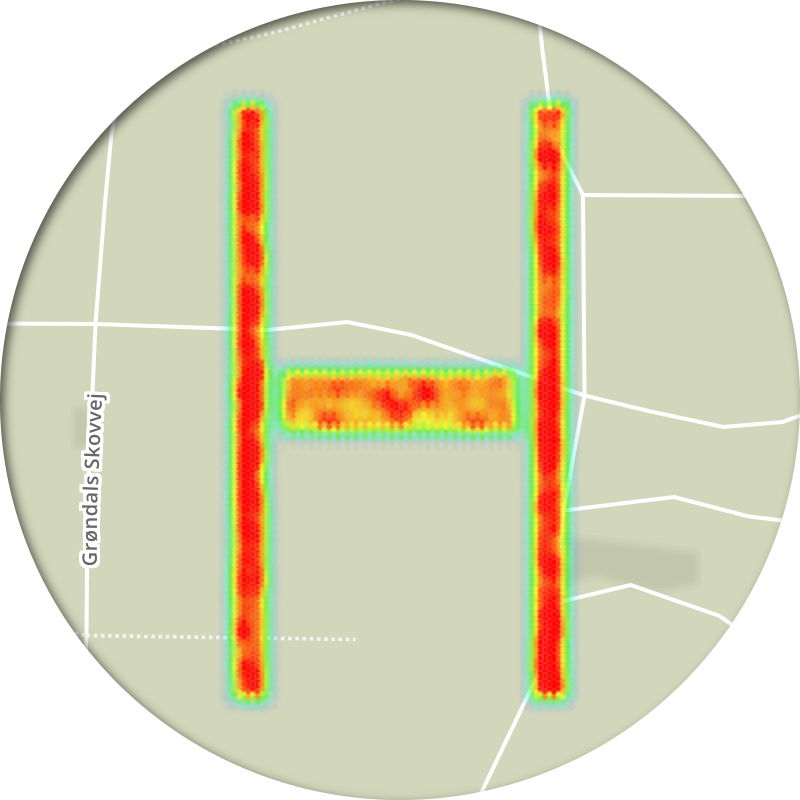
\includegraphics[width=0.5\textwidth]{titleLogo.PNG}
\end{center}


\vfill

% Bottom of the page
{\large May \nth{26}, 2016}

\end{center}
\end{titlepage}
